\documentclass[addpoints]{exam}
\usepackage{url}
\usepackage{amsmath,amsthm,enumitem}
\usepackage{graphicx}
\usepackage{qtree}
\usepackage[nodayofweek,level]{datetime}
\usepackage{color}
\usepackage{csquotes}
\usepackage{pgf, tikz}
\usetikzlibrary{arrows, automata}
\usepackage{algorithm,algpseudocode}
\newtheorem*{claim}{Claim}
\definecolor{qcolor}{rgb}{0, 0, 0.3}
\definecolor{acolor}{rgb}{0, 0, 0}
%\input myfonts
\qformat{Question \thequestion: \thequestiontitle\dotfill \textbf{[\totalpoints]}}
\pointname{}
\bonuspointname{}
\pointformat{[\bfseries\thepoints]}

\lhead{Gopal Menon (u0772360)}
\chead{\bf{HW3}}
\rhead{CS 6150 \today}
\headrule

\begin{document}

\section*{Collaborators}

Ben Nelson and I collaborated for this assignment.

\begin{questions}

\titledquestion{Negative edges}[4]
We saw that Dijkstra's algorithm (as such) requires all the edge weights to be non-negative in order to work. A student suggests a simple fix. Given a graph $G$ with negative weight edges (but no negative cycles), he suggests computing the least weight $w_{\min}$, and then adding $|w_{\min}|$ to all the edge weights. This would make all the weights non-negative. He claims that finding the shortest path on this new graph yields the shortest path in $G$ as well.

Is there something wrong in the reasoning above? Explain with an example (of some fixed size).

\begin{center}
  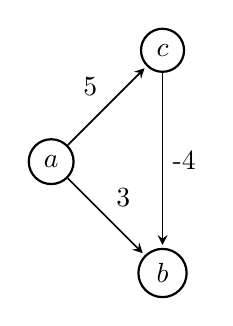
\begin{tikzpicture}[
            > = stealth, % arrow head style
            shorten > = 1pt, % don't touch arrow head to node
            auto,
            node distance = 2cm, % distance between nodes
            semithick % line style
        ]

        \tikzstyle{every state}=[
            draw = black,
            thick,
            fill = white,
            minimum size = 4mm
        ]

        \node[state] (a) {$a$};
        \node[state] (b) [below right of=a] {$b$};
        \node[state] (c) [above right of=a] {$c$};

        \path[->] (a) edge node {3} (b);
        \path[->] (a) edge node {5} (c);
        \path[->] (c) edge node {-4} (b);

  \end{tikzpicture}
\end{center}

Consider the case shown above where we need to find the shortest path from node $a$ to node $b$. The edge lengths are shown next to the edges. It can be seen that the shortest path from $a$ to node $b$ is through $c$, with a length of $5+(-4)=1$. The $1$-hop path from $a$ to $b$ is longer with a length of $3$. If we add $|w_{\min}| = |-4| =4$ to each each, we get the new graph shown below.

\begin{center}
  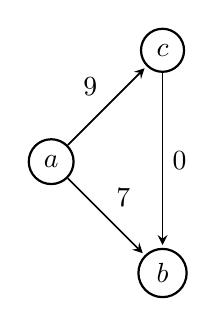
\begin{tikzpicture}[
            > = stealth, % arrow head style
            shorten > = 1pt, % don't touch arrow head to node
            auto,
            node distance = 2cm, % distance between nodes
            semithick % line style
        ]

        \tikzstyle{every state}=[
            draw = black,
            thick,
            fill = white,
            minimum size = 4mm
        ]

        \node[state] (a) {$a$};
        \node[state] (b) [below right of=a] {$b$};
        \node[state] (c) [above right of=a] {$c$};

        \path[->] (a) edge node {7} (b);
        \path[->] (a) edge node {9} (c);
        \path[->] (c) edge node {0} (b);

  \end{tikzpicture}
\end{center}

The shortest path now becomes the one directly from $a$ to $b$. The reason why this fix does not work is that $|w_{\min}|$ is added to each edge length and this may cause the shortest path in the original graph to no longer be the shortest one in the new graph with the changed edge weights, when the shortest path consists of multiple hops and the weight of each hop goes up by $|w_{\min}|$.

\titledquestion{Fattest path}[6]
Let $G$ be a directed graph in which every edge $e$ has a {\em thickness} $t_{e}$.  Given $u$ and $v$, find the path from $u$ to $v$ that maximizes the least-thick-edge on the path. [i.e., we want a path in which {\em every} edge is as thick as possible. Note that the length of the path does not matter.]

You will get partial credit if your algorithm runs in polynomial$(m, n)$ time ($m$ and $n$ are the number of edges and vertices, as usual). To receive full credit, it should run in $O((m+n)\log n)$ time. [{\em Hint: } You might want to modify Dijkstra's algorithm and use its run time analysis as a blackbox.]

\begin{minipage}{\linewidth}
  \begin{algorithm}[H]
    \caption{Modified Dijkstra's Algorithm}\label{Djk}
    \begin{algorithmic}[1]
      \Procedure{ModifiedDijkstra'sAlgorithm}{graph $G \{V, E\}$, thickness\_function $w$, start\_node $s$}
      	\State InitializeGraph($G$,$s$)
	\State $visited\_nodes\_set =\emptyset$
	\State $max\_priority\_q = G.V$ \Comment{based on vertex least thick edge}
	\While {$max\_priority\_q \neq \emptyset$}
		\State $a=Extract\_Max(max\_priority\_q)$
		\State $visited\_nodes\_set =  visited\_nodes\_set \cup \{a\}$
		\For {each vertex $b \in \{ \text{neighbors of  } a$\}}
			\State Relax($a, b, w$)
		\EndFor
	\EndWhile
      \EndProcedure    
      \Procedure{InitializeGraph}{graph $G \{V, E\}$, start\_node $s$}
	\For {each vertext $a \in G.V$}
		\State $a.least\_thick\_edge = 0$
		\State $a.predecessor = NIL$
	\EndFor
	\State $s.least\_thick\_edge =\infty$
      \EndProcedure
      \Procedure{Relax}{current\_node $a$, unvisited\_neighbor $b$, thickness\_function $w$}
	\If {$b.least\_thick\_edge < w(a,b)$}
		\State $b.least\_thick\_edge = w(a,b)$
		\State $b.predecessor = a$
	\EndIf
      \EndProcedure    
     \end{algorithmic}
  \end{algorithm}
\end{minipage}\\\\

The algorithm shown above is a slightly modified version of Dijkstra's Algorithm \cite{CLRS}. All the edges are first initialized with $0$ as the value of the least thick edge on the path that they are on. The starting node is initialized with $\infty$ for the least thick edge. The set of visited nodes is initially empty. A max priority queue based on the least thick edge for each vertex is used. The algorithm then repeatedly extracts the max node from the priority queue which will contain the frontier of unvisited nodes. The extracted node will be the one that lies on the path with the maximum least thickest edge. The running time of this algorithm will be the same \cite{CLRS} as the one for Dijkstra's Algorithm $O(n+m)\log n$.


\titledquestion{Answering distance queries}
Let $G = (V, E)$ be an {\em undirected} graph with all edge weights equal to $1$. Let $d(i,j)$ denote the length of the shortest path between $i$ and $j$.  Now, suppose we wish to answer queries from the user of the kind ``what is $d(u, v)$''? for different $u, v$.

One option is to compute answers to each query as it comes. This takes $O(m+n)$ time using BFS, as the graph is unweighted.  Another option is to solve the so-called All-Pairs-Shortest-Path (APSP) problem and store all the answers. This returns the answer in $O(1)$ time, but uses $O(n^2)$ additional memory -- which can be cumbersome for large graphs (think $n = 10^8$ -- common in real networks).  The goal of this problem is to see if there is middle ground, if we allow {\em an approximation}. The proposed algorithm does the following:

(pre-processing): choose a random subset $S$ of vertices (the size is specified later). For each $s \in S$, do a BFS and store the values $d(s, u)$ for all $u \in V$.

(query): at query time, given $u, v$, return $\min_{s \in S} \{ d(u, s) + d(v, s) \}$. 

\begin{parts}
\part[2] Prove that for any choice of $S$, the value we output for a query is $\ge d(u, v)$.  
\part[3] Suppose we obtain $S$ by randomly including every vertex of $U$ with probability $r/n$. (Thus the expected size of $S$ is $r$.) What are the expected pre-processing time and the memory usage of the algorithm?
\part[7] Suppose that $d(u,v) > 5n/r$ for some pair of vertices $u,v$.  Prove that with probability $> 0.99$, we obtain the right answer to the distance query. [{\em Hint:} consider the shortest path from $u$ to $v$ and the vertices on it.]
\end{parts}

The moral is that if $G$ is sparse, then by picking say $r = \sqrt{n}$, we can do much better than APSP, and get right distance values for all the ``long paths'' with high probability.

\begin{parts}

\part For any $u$ and $v$, the shortest path between them may or may not include a vertex that is in $S$. In the case that the shortest path between them includes a vertex in $S$, then  
$\min_{s \in S} \{ d(u, s) + d(v, s) \}$ will be equal to $d(u, v)$ for the case when the $s \in S$ that is in the shortest path between $u$ and $v$ is considered. For the case where the shortest path between $u$ and $v$ does not include a vertex in $S$, a path between $u$ and $v$ through any $s \in S$ will be longer than the shortest path between them. So we can conclude that the query will always output a value $\ge d(u, v)$.

\part Assuming that it takes constant time to decide whether to pick a vertex for the set $S$ or not, it will take $O(n)$ to look at every vertex and decide whether to include it or not. For every vertex $s \in S$, we would need to do a BFS in $O(m+n)$ time and then compute and store $d(s,u)$ for every $u \in V$. This will take a total of $O( n  + r \times (m+n)) = O(r \times (m+n))$ and will need $O(n \times |S|)=O(n \times r)$ storage to store the distance to each of the $n$ vertices from every vertex $s \in S$.

\part

\end{parts}

\titledquestion{Flows and cuts -- basics}
\begin{parts}
\part[5] As we mentioned in class, the image segmentation problem can be modeled as the following graph question:  let $G$ be a weighted undirected graph (weights non-negative), and let $S$ and $T$ be two subsets of the vertices. Find the smallest cut in $G$ that separates $S$ from $T$. In other words, find a subset of the edges with minimum total weight, such that after removing these edges, there is no path left from any $s \in S$ to $t \in T$.

(Note that in the standard formulation of cuts, $S$ and $T$ are singletons.) [{\em Hint: } find a way to use the min cut algorithm we saw in class in a blackbox manner.]

\part[5] {\bf Vertex disjoint paths.}  Let $G$ be an unweighted directed graph.  We saw how to construct multiple {\em edge}-disjoint paths from two given vertices $u$ and $v$ by simply viewing the graph as a flow network with every edge having a unit capacity, and finding the max flow from $u$ to $v$.

Now, suppose we wish to find the maximum number of paths possible from $u$ to $v$ that do not share any {\em vertices}.  Show how to cast this as a max-flow problem (of size polynomial in the size of $G$). 
\end{parts}

\titledquestion{Matchings}
Consider the matching problem that we have encountered before, but with {\em binary} weights. I.e., suppose we have $n$ children and $n$ gifts, and every child has a $0/1$ happiness value associated with each gift. The goal is to assign the gifts to the children, so as to maximize the total happiness. The question we wish to understand is: is there an assignment in which the total happiness is $n$? (I.e., can every child be assigned a gift to which he/she has a happiness value of $1$?)

\begin{parts}
\part[2] Let $\Gamma(i)$ denote the set of gifts for which child $i$ has a happiness value equal to $1$. One trivial case in which the total happiness cannot be made $n$ is if there is a set $R$ of children such that $\cup_{r \in R} \Gamma(r)$ has size $< |R|$. Give a short reason why this is so.

\part[5] Let us call a set $R$ as above a {\em trivial obstruction} (to the presence of an assignment of total happiness $n$). Prove that whenever the optimum total happiness is $<n$, such a trivial obstruction must exist. [{\em Hint:} use the max-flow min-cut theorem!] 
\end{parts}

\titledquestion{Matching games}
Alice and Bob play the following game: Alice starts by naming an actress A1. Bob must then name an actor B1 who has appeared in a movie with A1. Then Alice must name an actress A2 who appeared with B1, and so on. (Alice must always pick from the set of actresses, and Bob must pick from the set of actors.) The catch is that the players are not allowed to name anyone they have named already. The game ends and a player loses if he/she cannot name an actor/actress who hasn't been named already.

Suppose we are given as input a set of all ``allowed'' movies and their casts, and suppose that the total number of actresses is equal to the total number of actors. We can construct a bipartite graph between actresses and actors, in which there is an edge iff the two have appeared together in a movie. Let us call this graph $G$.  

\begin{parts}
\part[4] Prove that if $G$ has a perfect matching, then there is a winning strategy for Bob. (I.e., no matter how Alice plays, Bob can win.)
\part[7] If $G$ does {\em not} have a perfect matching, prove that Alice has a winning strategy.  [{\em Hint:} consider small examples; start with a maximum matching, and think of how Alice might want to start the play.]
\end{parts}

\end{questions}

\begin{thebibliography}{9}

\bibitem{CLRS} \enquote{24. Single-Source Shortest Paths.} \textit{Introduction to Algorithms}, by Thomas H. Cormen et al., MIT Press, 2009, pp. 648-662.

\end{thebibliography}

\end{document}
